\title{Extrapolating expected accuracies for recognition tasks}
\author{Charles Zheng, Rakesh Achanta and Yuval Benjamini}
\date{\today}

\documentclass[12pt]{article} 

% packages with special commands
\usepackage{amssymb, amsmath}
\usepackage{epsfig}
\usepackage{array}
\usepackage{ifthen}
\usepackage{color}
\usepackage{fancyhdr}
\usepackage{graphicx}
\usepackage{mathtools}
\usepackage{csquotes}
\usepackage{multirow}
\usepackage{xcolor}
\usepackage{chngcntr}
\usepackage{apptools}
\AtAppendix{\counterwithin{lemma}{section}}
\usepackage[backend=bibtex,style=authoryear]{biblatex}


\addbibresource{example.bib} % The filename of the bibliography

\newcommand\crule[3][black]{\textcolor{#1}{\rule{#2}{#3}}}

\definecolor{grey}{rgb}{0.5,0.5,0.5}
\definecolor{color1}{RGB}{128,13,13}
\definecolor{color2}{RGB}{70,128,13}
\definecolor{color3}{RGB}{13,128,128}
\definecolor{color4}{RGB}{70,13,128}

\begin{document}
\maketitle

\newcommand{\skone}{\mathcal{S}_{k_1}}
\newcommand{\sktwo}{\mathcal{S}_{k_2}}

\newcommand{\tr}{\text{tr}}
\newcommand{\E}{\textbf{E}}
\newcommand{\diag}{\text{diag}}
\newcommand{\argmax}{\text{argmax}}
\newcommand{\Cov}{\text{Cov}}
\newcommand{\Var}{\text{Var}}
\newcommand{\argmin}{\text{argmin}}
\newcommand{\Vol}{\text{Vol}}
\newcommand{\comm}[1]{}
\newcommand{\indep}{\rotatebox[origin=c]{90}{$\models$}}
\newcommand{\Cor}{\text{Cor}}
\newtheorem{theorem}{Theorem}[section]
\newtheorem{proposition}{Proposition}[section]
\newtheorem{corollary}{Corollary}[theorem]
\newtheorem{lemma}{Lemma}[section]
\newtheorem{definition}{Definition}[section]
\newcommand{\bZ}{\boldsymbol{Z}}
\newcommand{\bz}{\boldsymbol{z}}
\newcommand{\bx}{\boldsymbol{x}}
\newcommand{\bX}{\boldsymbol{X}}

\newcommand{\bH}{\boldsymbol{H}}


\begin{abstract}
The difficulty of multi-class classification generally increases with
the number of classes.  Using data from a subset of the classes, can
we predict how well a classifier will scale with an increased number
of classes?  Under the assumption that the classes are sampled
exchangeably, and under the assumption that the classifier is
generative (e.g. QDA or Naive Bayes), we show that the expected
accuracy when the classifier is trained on $k$ classes is the $k-1$st
moment of a \emph{conditional accuracy distribution}, which can be
estimated from data.  This provides the theoretical foundation for
performance extrapolation based on pseudolikelihood, unbiased
estimation, and high-dimensional asymptotics.  We investigate the
robustness of our methods to non-generative classifiers in simulations
and one optical character recognition example.
\end{abstract}

\section{Introduction}\label{sec:recog_tasks}

An algorithm that can use sensory information to automatically
 distinguish between multiple scenarios has increasingly many applications
 in modern life. Examples include detecting the speaker from his voice patterns, 
identifying the author from her written text, or labeling the object 
category from its image. All these examples can be described as recognition problems:
the algorithm observes an input $x$, and uses the classifier function $h$ to guess
the label $y$ from a discrete set $\mathcal{Y}$ of possible labels. 
In all applications described above, the space of potential labels is practically infinite.
But in any particular experiment, the number of different labels $k$ used would be finite.
A natural question, then, is how changing the number of 
possible labels affects the classification accuracy. 

More technically, we consider a sequence of classification
problems on finite label subsets
$|\mathcal{S}_k| < \cdots < |\mathcal{S}_K|, \mathcal{S}_i \subset \mathcal{Y}$,
where in the $k$-th task, one constructs the classification rule
$h^{(k)}:\mathcal{X} \to \mathcal{S}_k$.  Supposing that $(X, Y)$ have
a joint distribution, define the generalization accuracy for the
$k$-th problem as
\begin{equation}\label{eq:ga_k}
\text{GA}_k = \Pr[h^{(k)}(X) = Y|Y \in \mathcal{S}_k].
\end{equation}
The problem of \emph{performance extrapolation} is the following: using data
from only $\mathcal{S}_k$, can one predict the accuracy 
 for the larger label set $\mathcal{S}_K$?
Note that unlike other extrapolations from a smaller sample to a larger population, 
the classification problem becomes harder as the number of distractor classes
increases. 

Posing this question rigorously requires some effort. 
Within the statistics and machine learning literature, the usual
formalism for studying a recognition task is to pose it as a
\emph{multi-class classification} problem.  One delineates a finite
set of distinct entities which are to be recognized and distinguished,
which is the \emph{label set} $\mathcal{S}$. 

However, under this setup, it is usually assumed that the
label set $\mathcal{S}$ is a finite and specific set of categories, which is known in advance. [[Citations YB]] For human recognition systems, a fixed and finite label set is not always appropriate: humans can easily learn to recognize new objects. Similarly, we think about success of recognition systems as a property that is more general than accuracy on any individual set of classes. Therefore we need to extend the notion of accuracy to deal with multiple but related classification tasks.
[[Some citations of people doing mildly similar things YB: e.g. one-shot learning, transfer learning]] 


Accurate answers to this problem are not only of theoretical interest, but also have practical implications:

Example 1:

Facial recognition is an important technology with applications in
security and in social media, such as automatic tagging of photographs
on Facebook.  The basic problem is illustrated in Figure
\ref{fig:face_rec}: given a collection of tagged and cropped
photographs $\{(\vec{z}_j^{(i)}), y^{(i)}\}$, where $y^{(i)}$ is the
label, and $\vec{z}_j^{(i)}$ is a vector containing the numeric
features of the photograph (e.g. pixels), assign labels $y$ to
untagged photographs $\vec{z}_*$.  Here, the notation
$\vec{z}_j^{(i)}$ indicates the $j$th labelled photograph in the
database belonging to the $i$th individual. 

A client might want to run a facial recognition system
developed by lab A on their own database of individuals.  In this
case, there might be no overlap between the people in lab A's database
and the people in the client's database.  And yet, the client might
still expect the performance figures reported by lab A to be
informative of how well the recognition system will do on their own
database!
%One way to study the
%problem is to fit it into the multi-class classification framework,
%where the label set $\mathcal{Y}$ consists of all individuals in the
%data set, $\{y^{(1)},\hdots, y^{(k)}\}$.

\begin{figure}
\centering
\begin{tabular}{|c|ccc|c|}
\hline
Label & & Training & & Test\\ \hline
$y^{(1)}$=Amelia & 
  $\vec{z}_1^{(1)} = $
\includegraphics[scale = 0.2]{face_photos/Amelia_Vega_0001.png} &  
  $\vec{z}_2^{(1)} = $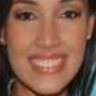
\includegraphics[scale = 0.2]{face_photos/Amelia_Vega_0002.png} &  
  $\vec{z}_3^{(1)} = $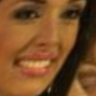
\includegraphics[scale = 0.2]{face_photos/Amelia_Vega_0003.png} &  
  $\vec{z}_*^{(1)} = $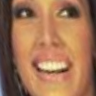
\includegraphics[scale = 0.2]{face_photos/Amelia_Vega_0004.png} \\ \hline
$y^{(2)}$=Jean-Pierre & 
  $\vec{z}_1^{(2)} = $
\includegraphics[scale = 0.2]{face_photos/Jean-Pierre_Raffarin_0001.png} &  
  $\vec{z}_2^{(2)} = $
\includegraphics[scale = 0.2]{face_photos/Jean-Pierre_Raffarin_0002.png} &  
  $\vec{z}_3^{(2)} = $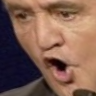
\includegraphics[scale = 0.2]{face_photos/Jean-Pierre_Raffarin_0003.png} &  
  $\vec{z}_*^{(2)} = $
\includegraphics[scale = 0.2]{face_photos/Jean-Pierre_Raffarin_0004.png} \\ \hline
$y^{(3)}$=Liza & 
  $\vec{z}_1^{(3)} = $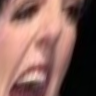
\includegraphics[scale = 0.2]{face_photos/Liza_Minnelli_0001.png} &  
  $\vec{z}_2^{(3)} = $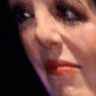
\includegraphics[scale = 0.2]{face_photos/Liza_Minnelli_0002.png} &  
  $\vec{z}_3^{(3)} = $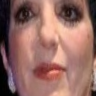
\includegraphics[scale = 0.2]{face_photos/Liza_Minnelli_0003.png} &  
  $\vec{z}_4^{(3)} = $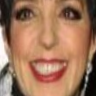
\includegraphics[scale = 0.2]{face_photos/Liza_Minnelli_0004.png} \\ \hline
$y^{(4)}$=Patricia & 
  $\vec{z}_1^{(4)} = $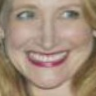
\includegraphics[scale = 0.2]{face_photos/Patricia_Clarkson_0001.png} &  
  $\vec{z}_2^{(4)} = $
\includegraphics[scale = 0.2]{face_photos/Patricia_Clarkson_0002.png} &  
  $\vec{z}_3^{(4)} = $
\includegraphics[scale = 0.2]{face_photos/Patricia_Clarkson_0003.png} &  
  $\vec{z}_4^{(4)} = $
\includegraphics[scale = 0.2]{face_photos/Patricia_Clarkson_0004.png} \\ \hline
\end{tabular}
\caption{Face recognition problem}
\label{fig:face_rec}
\end{figure}

Example 2: A neuroscientist is interested in how well the brain
  activity in various regions of the brain can discriminate between
  different classes of stimuli.  \cite{Kay2008a} obtained fMRI brain
  scans which record how a single subject's visual cortex responds to
  natural images. They wanted to know how well the brain signals could
  discriminate between different images. For a set of 1750
  photographs, they constructed a classifier which achieved over 0.75
  accuracy of classification. Based on exponential extrapolation, they
  estimate that it would take on the order of $10^{9.5}$ classes
  before the accuracy of the model drops below 0.10!  A theory of
  performance extrapolation could be useful for the purpose of making
  such extrapolations in a more principled way.
  
Both examples refer to the typical development of a recognition system. 
Recognition systems are first tested on small datasets, even 
if the longer-term goal is to deploy them on large datasets with many more classes.
The question is how much decay in the performance should we expect for the larger problem compared to the smaller problem. [Cite What Does Classifying...]
Theory for performance extrapolation may therefore
reveal models with bad scaling properties in the pilot stages of
development.

Our primary goal in this paper is to formulate this question, and
identify scenarios where answers are possible. 
The most important condition is that the smaller problem would be 
representative of the larger one. For simplicity, we
assume that both $\mathcal{S}_K$ and $\mathcal{S}_k$ are iid samples
from a population (or distribution) of labels. (Other sampling 
mechanisms would require some modification). 
The condition of i.i.d. sampling of labels ensures that the
separation of labels in a random set $\mathcal{S}_K$ can be inferred by
looking at the empirical separation in $\mathcal{S}_k$, and
therefore that some estimate of the achievable accuracy on
$\mathcal{S}_K$ can be obtained.

Our analysis considers a restricted set of classifiers,
\emph{marginal classifiers}, which train a separate model for each class. 
This convenient property allows us to
characterize the accuracy of the classifier by selectively
conditioning on one class at a time.  In section \ref{sec:extrapolation}, we use this
technique to reveal that the expected risk for classifying on the
label set $\mathcal{Y}_k$, for all $k$, is governed by a
specific function - the \emph{conditional risk} -  
that depends on the true distributions and the classifier. 
As long as one can recover the conditional risk
function $\bar{D}(u)$, one can compute the average risk for any number
of classes. 
  In section 5, we
empirically study the performance curves of classifiers on sequences
of classification tasks. 



The central theme of this thesis is the study of \emph{randomized
  classification}, which can be motivated as an extension of the
classical multi-class classification framework to accommodate the
possibility of growing or infinite label sets $\mathcal{Y}$. The basic
approach taken is to assume an infinite or even continuous label space
$\mathcal{Y}$, and then to study the problem of classification on
finite label sets $S$ which are randomly sampled from $\mathcal{Y}.$
This, therefore defines a \emph{randomized classification} problem
where the label set is finite but may vary from instance to instance.
One can then proceed to answer questions about the variability of the
performance due to randomness in the labels, or how performance
changes depending on the size of the random label set.


\subsection{Motivation}


The formalism of classification is inadequate for studying many
practical questions related to the generalizability of the facial
recognition system.  Using test data, we estimate the generalization
accuracy of a recognition system.  However, these estimated accuracies
apply only to the particular collection of individuals
$\{y^{(1)},\hdots, y^{(k)}\}$.  If we were to add a new individual
$y^{(k+1)}$ to the dataset, for instance, when photographs are
uploaded on Facebook containing a new user, this defines a totally new
classification problem because the expanded set of labels
$\{y^{(1)},\hdots, y^{(k+1)}\}$ defines a different response space
than the old set of labels $\{y^{(1)},\hdots, y^{(k)}\}$.  Yet, these
two classification problems are clearly linked.

The question of how to link performance between two different but
related classification tasks is an active area of research, known as
\emph{transfer learning}.  But while the two examples we just listed
might be considered as examples of transfer learning problems, the
current literature on transfer learning, as far as we know, does not
study the problem of \emph{mutating label sets}.  Therefore, to
address this new class of questions about the generalizability of the
recognition system, we need to formalize our notions of (a) what
constitutes a `recognition system' which can be applied to different
classification problems, and (b) what assumptions about the problem,
and what assumptions about the classifiers used, allow one to infer
performance in one classification problem based on performance in
another classification problem.

\section{Randomized classification}\label{sec:rc_motivation}


\subsection{Setup}

The randomized classification model we study has the following
features.  We assume that there exists an infinite, perhaps continuous, label space $\mathcal{Y}$ and a feature space $\mathcal{X} \in \mathbb{R}^p$.  
We assume there exists a prior distribution $\pi$ on the label space $\mathcal{Y}$.
And for each label $y \in \mathcal{Y}$,
there exists a distribution of features $F_y$. In other words, for a feature-label pair $(X, Y)$, the conditional distribution
of $X$ given $Y = y$ is given by $F_y$.  
%Furthermore, we assume that
%there exists a prior distribution $\pi$ on the label space $\mathcal{Y}$.

A random classification task can be generated as follows.  The
label set $\mathcal{S} = \{Y^{(1)},\hdots, Y^{(k)}\}$ is generated by
drawing labels $Y^{(1)},\hdots, Y^{(k)}$ i.i.d. from $\pi$.  
For each label, we sample a training set and a
test set.  The training set is obtained by sampling $r_{train}$ observations
$X_{j, train}^{(i)}$ i.i.d. from $F_{Y^{(i)}}$ for $j = 1,\hdots,
r_{train}$ and $i = 1,\hdots, k$.  The test set is likewise obtained by sampling $r$
observations $X_j^{(i)}$ i.i.d. from $F_{Y^{(i)}}$ for $j = 1,\hdots,
r$.  

We assume that the classifier $h(x)$ works by assigning a score to each label $y^{(i)} \in \mathcal{S}$, then choosing the label with the highest score.  That is, there exist real-valued \emph{score functions} $m_{y^{(i)}}(x)$ for each label $y^{(i)} \in \mathcal{S}$.
Since the classifier is allowed to depend on the training data, it is convenient to view it (and its associated score functions) as random.  We write $H(x)$ when we wish to work with the classifier as a random function, and likewise $M_y(x)$ to denote the score functions when they are considered as random.

For a fixed instance of the classification task with labels $\mathcal{S} = \{y^{(i)}\}_{i=1}^k$ and associated score functions $\{m_{y^{(i)}}\}_{i=1}^k$, recall the definition of the $k$-class generalization error \eqref{eq:ga_k}.  Assuming that there are no ties, it can be written in terms of score functions as
\[
\text{GA}_k(h) = \frac{1}{k} \sum_{i=1}^k  \Pr[m_{y^{(i)}}(X^{(i)}) = \max_j
m_{y^{(j)}}(X^{(i)})],
\]
where $X^{(i)} \sim F_{y^{(i)}}$ for $i =1,\hdots, k$.
However, when we consider the labels $\{Y^{(i)}\}_{i=1}^k$ and associated score functions to be random, the generalization accuracy also becomes a random variable.

Suppose we specify $k$ but do not fix any of the random quantities in the
classification task.  Then the $k$-class \emph{average generalization accuracy} of
a classifier is the expected value of the generalization accuracy $\text{GA}_k(H)$ resulting from a random set of $k$ labels, $Y^{(1)}, \hdots, Y^{(k)} \stackrel{iid}{\sim \pi}$, and their associated score functions:
\begin{align*}
\text{AGA}_k &= \frac{1}{k} \sum_{i=1}^k \Pr[M_{Y^{(i)}}(X^{(i)}) = \max_j
M_{Y^{(j)}}(X^{(i)})]
\\&= \Pr[M_{Y^{(1)}}(X^{(1)}) = \max_j M_{Y^{(j)}}(X^{(1)})].
\end{align*}
The last line follows from noting that all $k$ summands in the previous line are identical.
[The definition of average generalization accuracy is illustrated in Figure \ref{fig:average_risk}.]

\begin{figure}[h]
\centering
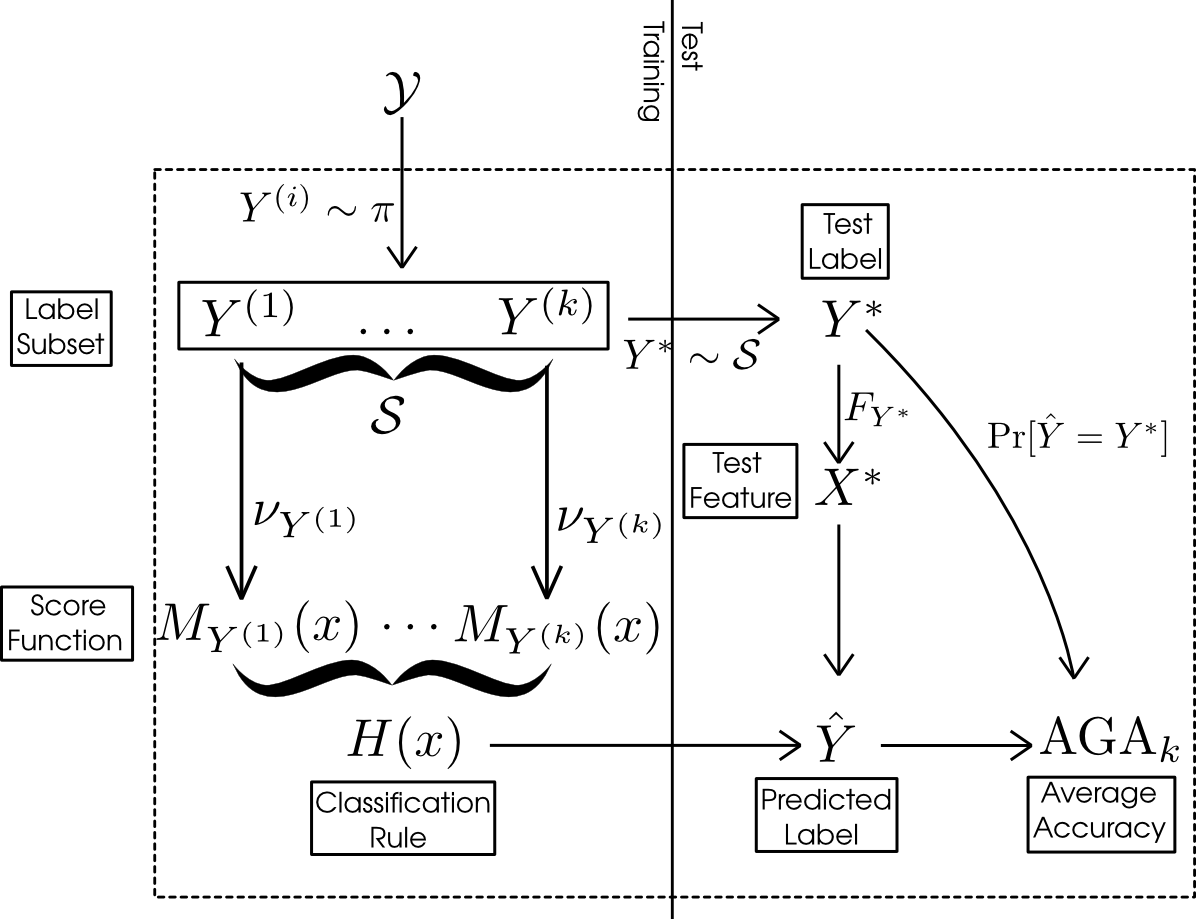
\includegraphics[scale = 0.3]{average_risk.png}
\caption{Average generalization accuracy}\label{fig:average_risk}
\end{figure}

\subsubsection{Marginal classifier}

In our analysis, we do not
want the classifier to rely too strongly on complicated interactions
between the labels in the set. We therefore propose the following
property of marginal separability for classification models:

\begin{definition}
The classifier $H(x)$ is called a \emph{marginal classifier} if the score 
function $M_{y^{(i)}}(x)$
only depends on the label $y^{(i)}$ and the class training set $X_{j, train}^{(i)}$.
\[M_{y^{(i)}}(x) = g(x; y^{(i)},X_{1, train}^{(i)},...,X_{r_{train}, train}^{(i)})\]
\end{definition}
This means that the score function for $y^{(i)}$ does not depend on other labels $y^{(j)}$ or their training 
samples.  Therefore, each $M_y$ can be considered to have been drawn from a distribution $\nu_y$.
Classes ``compete'' only through selecting the highest score, 
but not in constructing the score functions. 
The operation of a marginal classifier is illustrated in figure
\ref{fig:classification_rule}.


\begin{figure}[h]
\centering
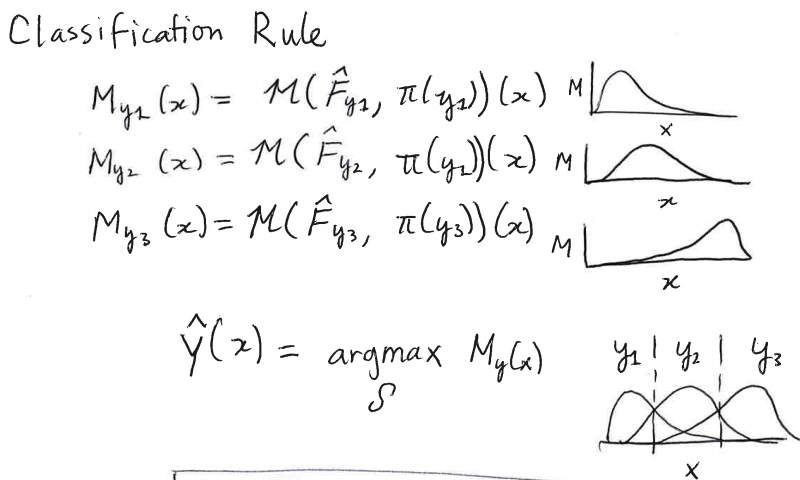
\includegraphics[scale = 0.4]{classification_rule.png}
\caption{Classification rule [to be updated]}\label{fig:classification_rule}
\end{figure}

The \emph{marginal} property allows us to prove
strong results about the accuracy of the classifier under
i.i.d. sampling assumptions.


\textbf{Comments:}
\begin{enumerate}
\item If $H$ is a marginal classifier then 
$M_{Y^{(i)}}$ is independent of $Y^{(j)}$ and $M_{Y^{(j)}}$ for $i \neq j$.
\item Estimated Bayes
classifier are a primary example of a marginal classifier. Let $\hat{f_y}$ be a density estimate of the feature distribution under label $y$ obtained from the
empirical distribution $\hat{F_y}$. Then, we can use the estimated
density to produce the score functions:
\[ m^{EB}_y(x) = \log(\hat{f_{y}}(x)).\]
The resulting empirical approximation for the Bayes classifier would be
\[ h^{EB}(x) = \text{argmax}_{y \in \mathcal{S}}(m^{EB}_y(x)).\]
\item Both the Quadratic Discriminant Analysis and the naive Bayes classifiers can be seen as specific instances of an estimated Bayes classifier
\footnote{QDA is the special case of the estimated Bayes classifier when $\hat{f_y}$ is obtained as
the multivariate Gaussian density with mean and covariance parameters estimated from the data.
Naive Bayes is the estimated Bayes classifier when $\hat{f_y}$ is obtained as the product of estimated componentwise marginal distributions
of $p(x_i|y)$}. 
For QDA, the score function is
given by
\[
m_y^{QDA}(x) = -(x - \mu(\hat{F}_y))^T \Sigma(\hat{F}_y)^{-1} (x-\mu(\hat{F}_y)) - \log\det(\Sigma(\hat{F}_y)),
\]
where $\mu(F) = \int y dF(y)$ and $\Sigma(F) = \int (y-\mu(F))(y-\mu(F))^T dF(y)$.
In Naive Bayes, the score function is
\[
m^{NB}_y(x) = \sum_{j=1}^p \log \hat{f}_{y, j}(x),
\]
where $\hat{f}_{y, j}$ is a density estimate for the $j$-th component of
$\hat{F}_y$.
\item For some classifiers, $M_y$ is a deterministic function of $y$ (and therefore $\nu_y$ is degenerate). A prime example is when exists fixed or pre-trained embeddings $g, \tilde{g}$ that map labels $y$ and features $x$ into
 $R^p$. Then 
\begin{equation}
M_y^{embed} = -\|g(y) - \tilde{g}(x)\|_2.
\end{equation}
This describes, for example, a 1-nearest neighbor classifier.
\item There are many classifiers which do not satisfy the marginal property, such as multinomial logistic regression, multilayer neural networks, decision trees, and k-nearest neighbors.
\end{enumerate}

\emph{Notational remark.}  Henceforth, we shall relax the assumption that the classifier $H(x)$ is based on a training set.  Instead, we assume that there exist score functions $\{M_{Y^{(i)}}\}_{i=1}^k$ associated with the random label set $\{Y^{(i)}\}_{i=1}^k$, and that the score functions $M_{Y^{(i)}}$ are independent of the test set.  The classifier $H(x)$ is marginal if and only if $M_{Y^{(i)}}$ are independent of both $Y^{(j)}$ and $M_{Y^{(j)}}$ for $j \neq i$.

\subsection{Estimation of average accuracy}\label{sec:estimation_average_accuracy}

Suppose we have test data for a classification task with $k_1$ classes.  That is, we have a label set $\mathcal{S}_{k_1} =
\{y^{(i)}\}_{i=1}^{k_1}$ and its associated set of score functions
 $M_{y^{(i)}}$, as well as test observations $(x_1^{(i)},\hdots, x_{r}^{(i)})$ for $i =
1,\hdots, k_1$.  What would be the predicted accuracy for 
a new randomly sampled set of $k_2 \leq k_1$ labels? 

Note that $\text{AGA}_{k_2}$
is the expected value of the accuracy on the
new set of $k_2$ labels.  Therefore, any unbiased estimator of $\text{AGA}_{k_2}$ will be an unbiased predictor for the accuracy on the new set.

Let us start with the case $k_2 = k_1 = k$.  For each test observation $x_j^{(i)}$, define the ranks of the candidate classes $\ell = 1,\hdots, k$ by
\[
R_{j}^{i, \ell} = \sum_{s = 1}^k I\{m_{y^{(\ell)}}(x_j^{(i)}) \geq m_{y^{(s)}}(x_j^{(i)})\}.
\]
The test accuracy is the fraction of observations for which the correct class also has the highest rank
\begin{equation}\label{eq:test_risk}
\text{TA}_k = \frac{1}{r k} \sum_{i=1}^{k} \sum_{j=1}^{r} I\{R_j^{i,i} = k\}.
\end{equation}
Taking expectations over both the test set and the random labels, the expected value of the test accuracy is $\text{AGA}_k$; hence, $\text{TA}_k$ provides the desired estimator.

Next, let us consider the case where $k_2 < k_1$.  
Consider label set $\mathcal{S}_{k_2}$ obtained
by sampling $k_2$ labels uniformly without replacement from
$\mathcal{S}_{k_1}$. Since $\mathcal{S}_{k_2}$ is unconditionally an i.i.d. sample from 
the population of labels $\pi$, the test accuracy of $\mathcal{S}_{k_2}$ is an unbiased estimator of $\text{AGA}_{k_2}$.
However, we can get a better unbiased estimate of
$\text{AGA}_{k_2}$ by averaging over all the possible subsamples
$\mathcal{S}_{k_2} \subset \mathcal{S}_{k_1}$. 
This defines the average test accuracy over subsampled tasks, $\text{ATA}_{k_2}$.

\emph{Remark.}
Na\"{i}vely, computing $\text{ATA}_{k_2}$ requires us to train and evaluate
${k_1}\choose{k_2}$ classification rules.  However, for marginal classifiers, retraining the classifier is not necessary.
Looking at the rank $R_{j}^{i,i}$ of the correct label $i$ for $x_j^{(i)}$,
allows us to determine how many subsets $\mathcal{S}_2$
will result in a correct classification. Specifically,
there are $R_{j}^{i,i} - 1$ labels with a lower score than the correct
label $i$.  Therefore, as long as one of the classes in
$\mathcal{S}_2$ is $i$, and the other $k_2-1$ labels are from the set of
$R_{j}^{i,i}-1$ labels with lower score than $i$, the classification of
$x_j^{(i)}$ will be correct.  This implies that there are
${R_{j}^{i,i}-1}\choose{k_2-1}$ such subsets $\mathcal{S}_2$ where
$x_j^{(i)}$ is classified correctly, and therefore the average test risk for all ${k_1}\choose{k_2}$ subsets $\mathcal{S}_2$ is
\begin{equation}\label{eq:avtestrisk}
\text{ATA}_{k_2} = \frac{1}{{{k_1}\choose{k_2}}}\frac{1}{r k_2} \sum_{i=1}^{k_1} \sum_{j=1}^{r} {{R_{j}^{i,i}-1}\choose{k_2-1}}.
\end{equation}

\subsection{Toy Example: Bivariate normals}

Let us illustrate these ideas using a toy example.
Let $(Y, X)$ have a bivariate normal joint distribution,
\[
(Y, X) \sim N\left(\begin{pmatrix}0 \\0\end{pmatrix}, \begin{pmatrix}1 & \rho \\ \rho & 1\end{pmatrix}\right),
\]
as illustrated in figure \ref{fig:toy1}(a).
Therefore, for a given randomly drawn label $Y$, the conditional
distribution of $X$ for that label is univariate normal with mean $\rho Y$ and variance $1-\rho^2$:
\[
X|Y = y \sim N(\rho Y, 1-\rho^2).
\]
Supposing we draw $k = 3$ labels $y_1,y_2, y_3$, the classification
problem will be to assign a test instance $X^*$ to the correct label.
The test instance $X^*$ would be drawn with equal probability from one of three conditional distributions
$ X | Y=y^{(i)}$, as illustrated in figure \ref{fig:toy1}(b, top).
The Bayes rule assigns $X^*$
to the class with the highest density $p(x|y_i)$, as illustrated by
figure \ref{fig:toy1}(b, bottom): it is therefore a marginal classifier, with
score function
\[
M_{y^{(i)}}(x) = \log(p(x|y^{(i)})) = -\frac{(x - \rho y)^2}{2(1-\rho^2)}  + \text{const.}
\]

\begin{figure}[h]
\centering
\begin{tabular}{cc}
\multirow{3}{*}{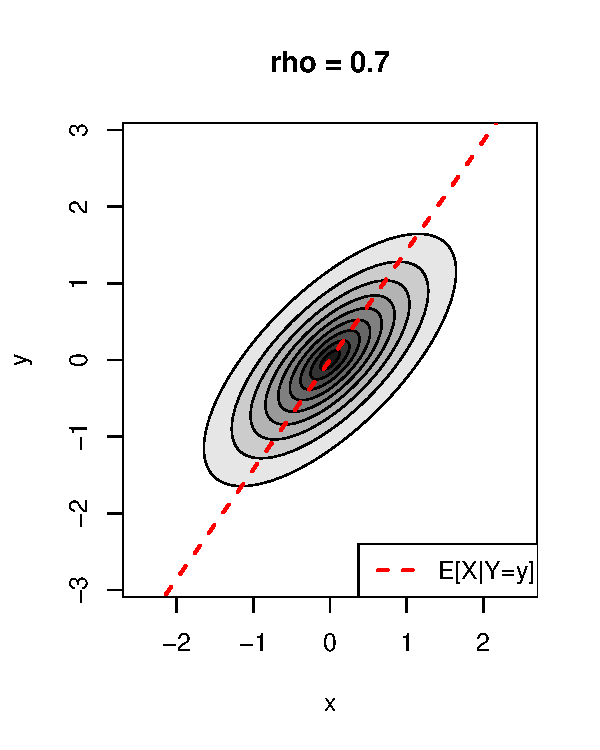
\includegraphics[scale = 0.5, clip = true, trim = 0 0 0 0.5in]{illus_rho_0_7.pdf}} & \\
& 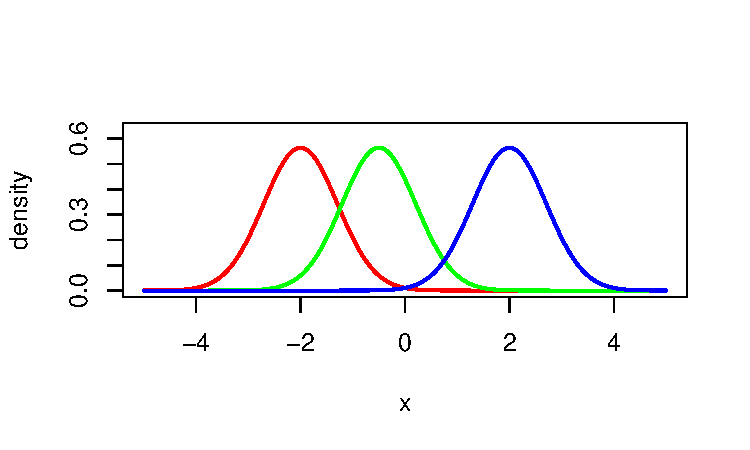
\includegraphics[scale = 0.5, clip = true, trim = 0 0.8in 0 0.8in]{illus_example1a.pdf}\\
 &  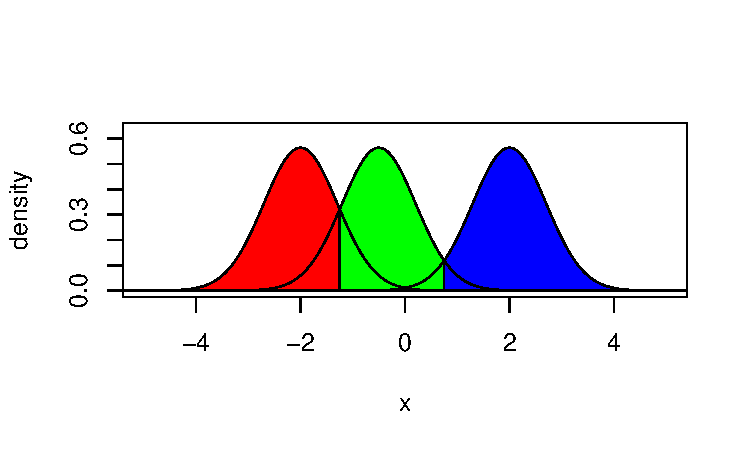
\includegraphics[scale = 0.5, clip = true, trim = 0 0 0 0.5in]{illus_example1b.pdf}\\
(a) & (b)
\end{tabular}

\caption{
(a) The joint distribution of $(X, Y)$ is bivariate normal with correlation $\rho = 0.7$.
(b) A typical classification problem instance from the bivariate normal model with $k = 3$ classes.
Top: the conditional density of $X$ given label $Y$, for $Y = \{y_1, y_2, y_3\}$.
Bottom: the Bayes classification regions for the three classes.}\label{fig:toy1}
\end{figure}

For this model, the generalization accuracy of the Bayes rule for any label set $\{y^{(1)},\hdots, y^{(k)}\}$ is given by
\begin{align*}
\text{GA}_k(y_1,\hdots, y_k) &= \frac{1}{k}\sum_{i=1}^k \Pr_{X \sim p(x|y_i)}[p(X|y_i) = \max_{j=1}^k p(X|y_j)]
\\&= \frac{1}{k}\sum_{i=1}^k \Phi\left(\frac{y^{[i+1]} - y^{[i]}}{2\sqrt{1-\rho^2}}\right) - \Phi\left(\frac{y^{[i-1]} - y^{[i]}}{2\sqrt{1-\rho^2}}\right)
\end{align*}
where $\Phi$ is the standard normal cdf, $y^{[1]} < \cdots < y^{[k]}$ are the sorted labels, and $y^{[0]} = -\infty$ and $y^{[k+1]} = \infty$.
We numerically computed $\text{GA}_k(y_1,\hdots, y_k)$ for randomly
drawn labels $Y_1,\hdots, Y_k \stackrel{iid}{\sim} N(0, 1)$; the
distributions of $\text{GA}_k$ for $k = 2,\hdots, 10$
are illustrated in figure \ref{fig:toy2}.  The mean of the distribution of $\text{GA}_k$ is the $k$-class average risk,
$\text{AGA}_k$. The theory
presented in the next section deals with how to analyze the
average risk $\text{AGA}_k$ as a function of $k$. 


\begin{figure}[h]
\centering
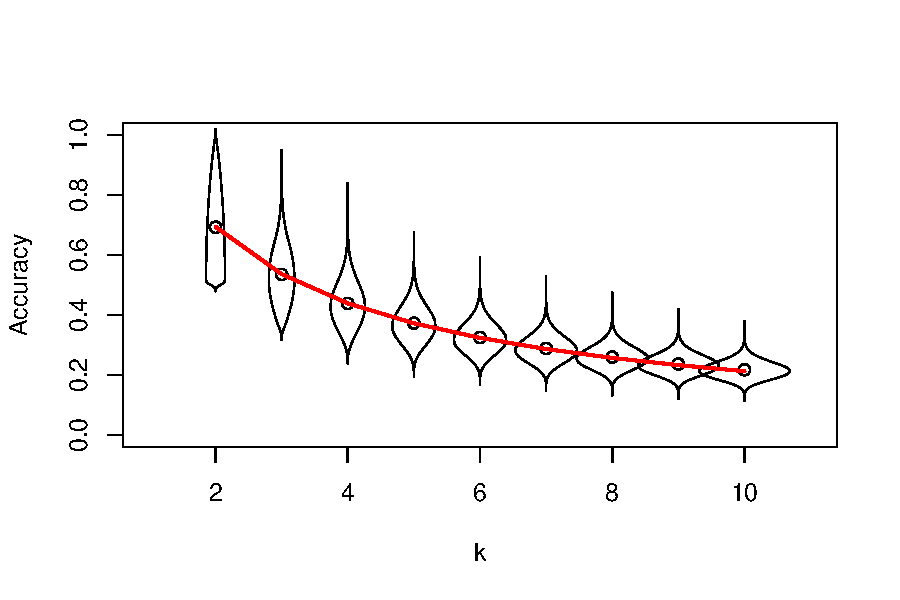
\includegraphics[scale = 0.7, clip = true, trim = 0 0 0 0.5in]{illus_err_0_7.pdf}

\caption{[change figure]The distribution of the classification risk for $k = 2,3,\hdots, 10$ for the bivariate normal model with $\rho = 0.7$.
Circles indicate the average classificatin risk; the red curve is the theoretically computed average risk.}\label{fig:toy2}
\end{figure}
\section{Extrapolation}

The section is organized as follows.  We begin by introducing an explicit formula for the average accuracy $\text{AGA}_{k}$.  The formula reveals that $\text{AGA}_{k}$ is determined by moments of a one-dimensional function $\bar{D}(u)$.
Through this formula, therefore, we can infer through subsample accuracies 
estimates of $\bar{D}(u)$. 
These estimates allow us to extrapolate the average generalization
accuracy to an arbitrary number of labels.

Furthermore, the formula links 
Therefore, we propose a basis-function repestimate $\text{AGA}_{k}$ by estimating this
function, and  through non-parameteric 
estimation of the unknown function.  This allows the
development of a class of unbiased estimators of $\bar{D}(u)$,
presented in section \ref{sec:extrapolation_estimation} given the
assumption of a known parametric form for $\bar{D}(u)$.  
%We analyze
%the performance of the estimator in both the well-specified and
%misspecified case.  
We demonstrate our method to a face-recognition
example in section \ref{sec:extrapolation_example}.




\subsection{Analysis of average risk}

The result of our analysis is to expose the average accuracy
$\text{AGA}_{k}$ as the weighted average of a function
$\bar{D}(u)$, where $\bar{D}(u)$ is independent of $k$, and where $k$
only changes the weighting.  The result is stated as follows.

\begin{theorem}\label{theorem:avrisk_identity}
Suppose $\pi$, $\{F_y\}_{y \in \mathcal{Y}}$ and score functions $M_y$ satisfy the tie-breaking condition.  Then, there exists a cumulative distribution function $\bar{D}(u)$ defined on the interval $[0,1]$ such that
\begin{equation}\label{eq:avrisk_identity}
\text{AGA}_{k} = 1 - (k-1) \int \bar{D}(u) u^{k-2} du.
\end{equation}
\end{theorem}

The tie-breaking allows us
to neglect specifying the case when
margins are tied.
\begin{definition}
\emph{Tie-breaking condition}: for all $x \in \mathcal{X}$,
$M_Y(x) \neq M_{Y'}(x)$
with probability one for $Y, Y'$ independently drawn from $\pi$.
\end{definition}
In practice, one can simply break ties randomly,
which is mathematically equivalent to adding a small amount of random
noise $\epsilon$ to the function $\mathcal{M}$.



As we can see from Figure \ref{fig:average_risk}, the average accuracy is
obtained by averaging over four randomizations:
\begin{enumerate}
\item[A1.] Drawing the label subset $\mathcal{S}=\{Y^{(1)},\hdots,Y^{(k)}\}$.
\item[A2.] Training the associated score functions, $M_{Y^{(1)}},\hdots, M_{Y^{(k)}}.$
\item[A3.] Drawing $Y^*$ uniformly at random from $\mathcal{S}$.
\item[A4.] Drawing $X^*$ from $F_{Y^*}$.
\end{enumerate}


Our strategy is to analyze the average accuracy by
means of \emph{conditioning on} the true label and its score function, $(y^*, m_{y^*})$, and the test feature $x^*$
while \emph{averaging} over all the other random variables.  Define
the \emph{conditional accuracy} $\text{CondA}_k(m_{y^*}, x^*)$ as
\[
\text{CondA}_k(m_{y^*}, x^*) = \Pr[\max_{y \in \mathcal{S}} M_y(X^*) = M_{Y^*}(X^*) | X^* = x^*, M_{Y^*} = m_{y^*}].
\]
Figure \ref{fig:conditional_risk} illustrates the variables which are
fixed under conditioning and the variables which are randomized.
Compare to figure \ref{fig:average_risk}.

Without loss of generality, we can write the label subset $\mathcal{S}
= \{Y^*, Y^{(1)},\hdots, Y^{(k-1)}\}$.  Note that due to independence,
$Y^{(1)},\hdots, Y^{(k-1)}$ are still i.i.d. from $\pi$ even
conditioning on $X^*=x^*$ and $M_{Y^*} = m_{y^*}$. Therefore, the conditional risk can be
obtained via the following alternative order of randomizations:
\begin{enumerate}
\item[C0.] 
Fix $y^*, m_{y^*},$ and $x^*$.
\item[C1.]
Draw the \emph{incorrect labels} $Y^{(1)},\hdots, Y^{(k-1)}$ i.i.d. from
$\pi$.  (Note that $Y^{(i)} \neq y^*$ with probability 1 due to the
continuity assumptions on $\mathcal{Y}$ and $\pi$.)
\item[C2.]
Train the score functions for the incorrect labels
$M_{Y^{(1)}},\hdots, M_{Y^{(k-1)}}$.  This determines
\[
\hat{Y} = \argmax_{y \in \mathcal{S}} M_y(x^*)
\]
and hence, whether or not the classification is correct for $(x^*, y^*)$
\end{enumerate}
Compared to four randomization steps for the average risk, we have
essentially conditioned on steps A3 and A4 and randomized over steps
A1 and A2.

\begin{figure}[h]
\centering
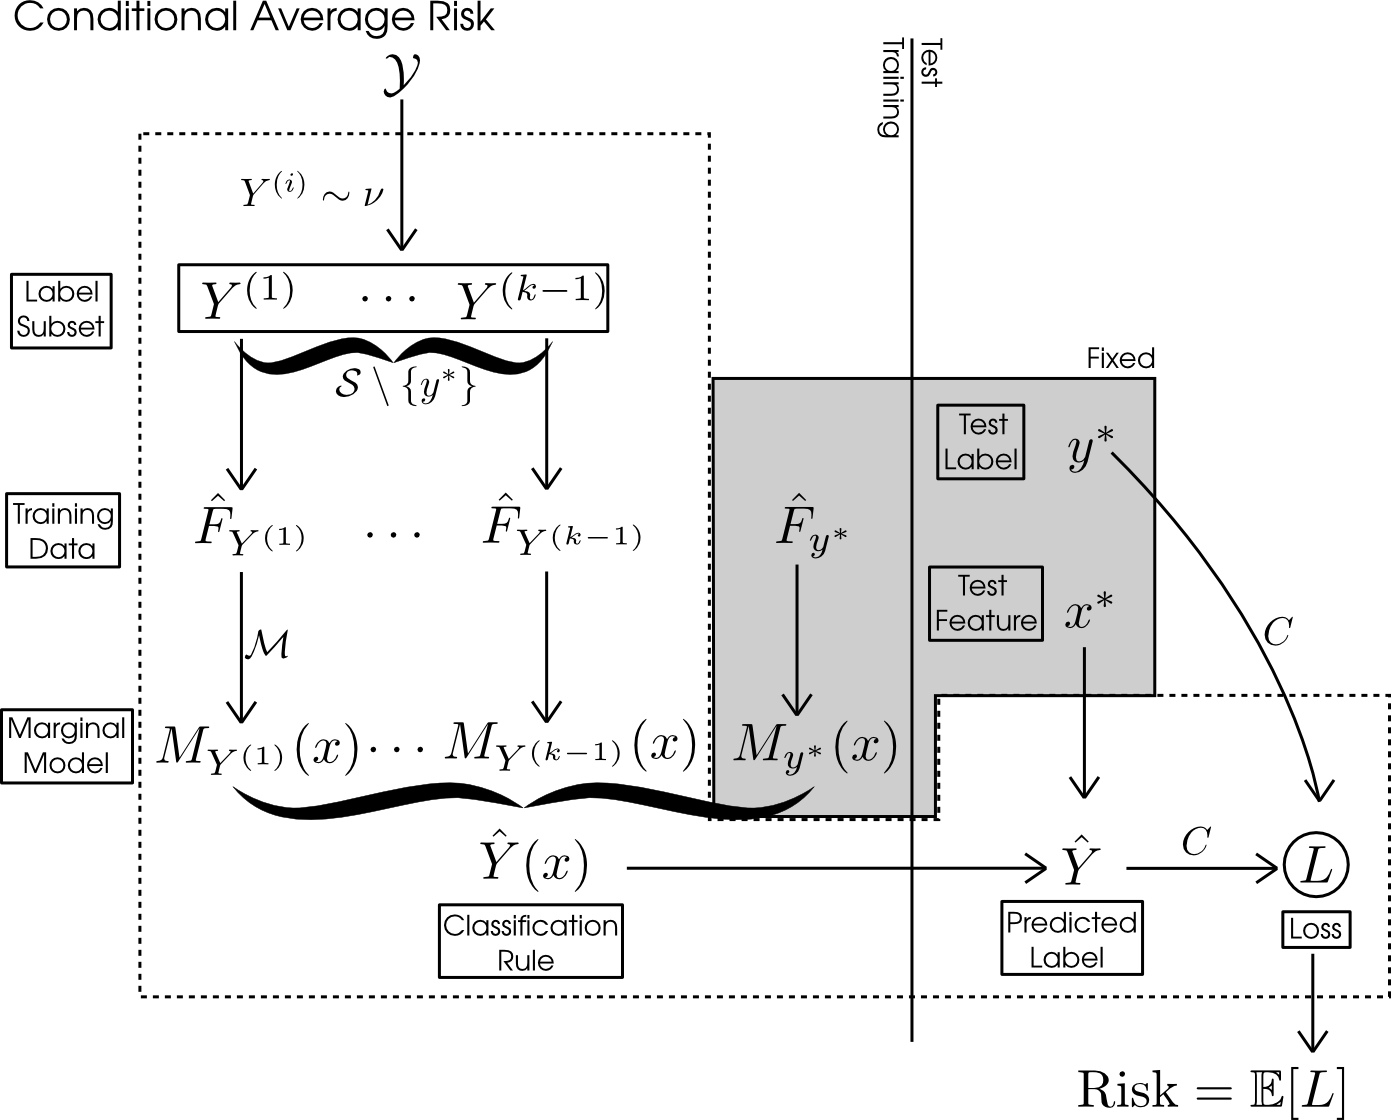
\includegraphics[scale = 0.3]{conditional_risk.png}
\caption{Conditional accuracy}\label{fig:conditional_risk}
\end{figure}

We begin by considering the \emph{two-class} conditional accuracy.
In addition to the true label $y^*$ and its score function $m_{y^*}$, 
we have one single incorrect label $Y$ with its associated score function, $M_Y$.  
Then we denote by $U_{x^*}(m_{y^*})$ the conditional accuracy 
\begin{equation}\label{eq:U_function}
U_{x^*}(m_{y^*}) = \Pr[m_{y^*}(x^*) > M_Y(x^*)].
\end{equation}
Here, the classification is correct if and
only if \[m_{y^*}(x^*) \geq M_Y(x^*),\] that is, if the score of the
incorrect class is larger than the score of the correct class for
observation $x^*$.
See also figure \ref{fig:U_function} for an graphical illustration of
the definition.

\begin{figure}[h]
\centering
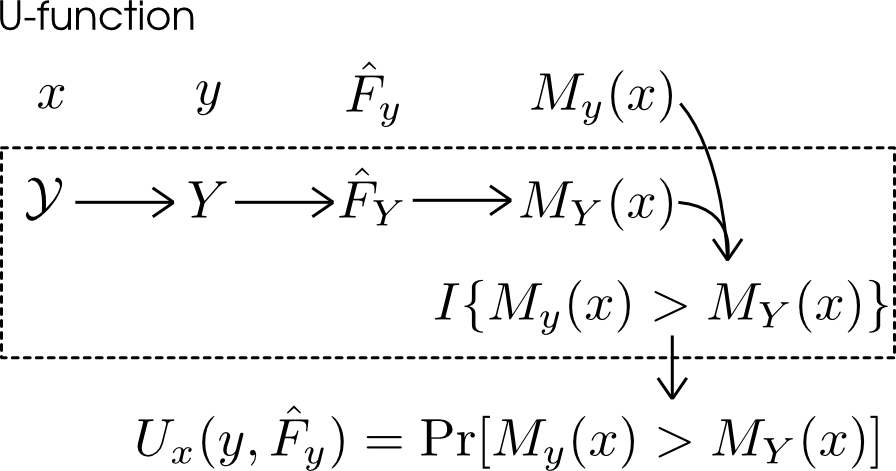
\includegraphics[scale = 0.4]{U_function.png}
\caption{U-functions}\label{fig:U_function}
\end{figure}

An important property of the U-function, and the basis for its name,
is that the random variable $U_X(M_Y)$ for $Y \sim \pi$ and $X \sim F_Y$ and $M_Y \sim \nu_Y$, is uniformly distributed
conditional on $X=x$, for all fixed $x \in \mathcal{X}$.  This is
proved in the following Lemma.

\begin{lemma}\label{lemma:U_function}
Suppose $\pi$, $\{M_y\}_{y \in \mathcal{Y}}$ and marginal classifier
$\mathcal{F}$ satisfy the tie-breaking condition.  Take $x \in \mathcal{X}$.  Defining
$U_x(m_y)$ as in \eqref{eq:U_function}, and defining the
random variable $U$ by
\[U = U_X(M_Y)\]
for $Y \sim \pi$, $X \sim F_Y$, and $M_Y \sim \nu_Y$.  Then
the conditional distribution of $U$ given $X = x$ for any $x \in
\mathcal{X}$ is uniform on $[0,1]$, i.e.
\[
\Pr[U \leq u|X =x] = \text{min}\{u, 1\}.
\]
\end{lemma}

\textbf{Proof of Lemma.}

%Define the variable $Z = \mathcal{M}(\hat{F}_Y)(x)$ for $Y \sim \pi$.
%By the tie-breaking condition, $Z$ has a continuous density on $[0,1]$.
%Consider the survivor function of $Z$, $g(z) = \Pr[Z \geq z]$.  From
%the definition \eqref{eq:U_function}, we see that 
%\[
%U = g(\mathcal{M}(\hat{F}_Y)(x)) = g(Z).
%\]
%Now note that the survivor function of any continuous random variable,
%when applied to itself, is uniformly distributed.

The result follows from the fact that the conditional probability
$\Pr[W > W'|W]$ is uniformly distributed for any $W, W'$ which are
i.i.d. with a continuous distribution.  

Define $Z = M_Y(x)$ and $Z' =
M_{Y'}(x)$ for $Y, Y' \stackrel{i.i.d.}{\sim} \pi$.
Then, conditional on $X = x$, we have
\[
U = \Pr[Z > Z'|Z].
\]
The tie-breaking conditional implies that $Z$ has a continuous
distribution, so therefore $U$ is uniformly distributed conditional on
$X = x$.  $\Box$

Now, we will see how the U-function allows us to understand the
$k$-class case.  Suppose we have true label $y^*$ and incorrect labels
$Y^{(1)},\hdots, Y^{(k-1)}$.  Note that the U-function
$U_{x^*}(m_y)$ is monotonic in $m_y(x^*)$.  Therefore,
\[
\hat{Y} = \argmax_{y \in \mathcal{S}} M_y(x^*) = \argmax_{y \in \mathcal{S}} U_{x^*}(M_y).
\]
Therefore, we have a correct classification if and only if the U-function value for the correct label
is greater than the maximum U-function values for the incorrect labels:
\[
\Pr[\hat{Y} = y^*] = \Pr[U_{x^*}(m_{y^*}) > \max_{i=1}^{k-1} U_{x^*}(M_{Y^{(i)}})] =  \Pr[u^* > U_{max}].
\]
where $u^* = U_{x^*}(m_{y^*})$ and $U_{max, k-1}
= \max_{i=1}^{k-1} U_{x^*}(M_{Y^{(i)}})$.  But now,
observe that we know the distribution of $U_{max, k-1}$.  Since
$U_{x^*}(M_{Y^{(i)}})$ are i.i.d. uniform, we know that
\begin{equation}\label{eq:umax_beta}
U_{max, k-1} \sim \text{Beta}(k-1, 1). 
\end{equation}

Therefore, in the general case, the conditional accuracy is
\[
\text{CondAcc}_k((y^*, \hat{F}_{y^*}), x^*) = \Pr[U_{max} \leq u^*] = \int_0^{u^*} (k-1) u^{k-2} du.
\]
Now the average accuracy can be obtained by integrating over the
distribution of $U^* = U_{X^*}(Y^*, \hat{F}_{Y^*})$, which we state in
the following proof of theorem \ref{theorem:avrisk_identity}.

\noindent\textbf{Proof of Theorem \ref{theorem:avrisk_identity}}.
We have
\begin{align*}
\text{AGA}_{k,r} &= \E[\int_0^{U^*} (k-1) u^{k-2} du] 
\\&= \E[\int_0^1 I\{u \leq U^*\} (k-1) u^{k-2} du ]
\\&= (k-1) \int_0^1 \Pr[U^* \geq u] u^{k-2} du.
\end{align*}
Or equivalently,
\[
\text{AGA}_{k, r}((y^*, \hat{F}_{y^*}), x^*) = 1 - (k-1) \int \bar{D}(u) u^{k-2} du.
\]
where $\bar{D}(u)$ denotes the cumulative distribution function of $U^*$ on $[0,1]$:
\begin{equation}\label{eq:Kbar}
\bar{D}(u) = \Pr[U_{X^*}(Y^*, \hat{F}_{y^*}) \leq u].
\end{equation}
We have expressed the average risk expressed as a weighted integral of
a certain function $\bar{D}(u)$ defined on $u \in [0,1]$.  We have
clearly isolated the part of the average risk which is independent of
$k$--the univariate function $\bar{D}(u)$, and the part which is
dependent on $k$--which is the density of $U_{max}$.

In section \ref{sec:extrapolation_estimation}, we will develop
estimators of $\bar{D}(u)$ in order to estimate the $k$-class average
risk.

Having this theoretical result allows us to understand how the
expected $k$-class risk scales with $k$ in problems where all the
relevant densities are known.  However, applying this result in
practice to estimate $\text{AGA}_k$ requires some means of
estimating the unknown function $\bar{D}$--which we discuss in the
following.

\subsection{Estimation}\label{sec:extrapolation_estimation}

Now we address the problem of estimating $\text{AGA}_{k_2, r_1}$ from
data.  As we have seen from Theorem \ref{theorem:avrisk_identity}, the
$k$-class average accuracy of a marginal classifier $\mathcal{M}$ is a
functional of a object called $\bar{D}(u),$ which depends marginal
model $\mathcal{M}$ of the classifier, the joint distribution of
labels $Y$ and features $X$ when $Y$ is drawn from the population
density $\pi$.

Therefore, the strategy we take is to attempt to estimate $\bar{D}$
for the given classification model, and then plug in our estimate of
$\bar{D}$ into the integral \eqref{eq:avrisk_identity} to obtain an
estimate of $\text{AGA}_{k_2, r_{train}}$.

Having decided to estimate $\bar{D}$, there is then the question of
what kind of model we should assume for $\bar{D}$.  In this work, we
assume that some parametric model\footnote{While a
nonparametric approach may be more ideal, we leave this to future work.} is available for $\bar{D}$.

Let us assume the linear model
\begin{equation}\label{eq:linearKu}
\bar{D}(u) = \sum_{\ell = 1}^m \beta_\ell h_\ell(u),
\end{equation}
where $h_\ell(u)$ are known basis functions, and $\beta$ are the model
parameters to be estimated. We can obtain \emph{unbiased} estimation
of $\text{AGA}_{k_2, r_{train}}$ via the unbiased estimates of
$k$-class average risk obtained from \eqref{eq:avtestrisk}.

If we plug in the assumed linear model \eqref{eq:linearKu} into the
identity \eqref{eq:avrisk_identity}, then we get
\begin{align}
1 - \text{AGA}_{k, r_{train}} &= (k-1)\int \bar{D}(u) u^{k-2} du
\\&= (k-1)\int_0^1 \sum_{\ell = 1}^m \beta_\ell h_\ell(u) u^{k-2} du
\\&= \sum_{\ell = 1}^m \beta_\ell H_{\ell,k} \label{eq:avrisk_linear}
\end{align}
where
\begin{equation}
H_{\ell,k} = (k-1) \int_0^1 h_\ell(u) u^{k-2} du.
\end{equation}
The constants $H_{\ell, k}$ are moments of the basis function
$h_\ell$: hence we call this method the \emph{moment method.}  Note
that $H_{\ell, k}$ can be precomputed numerically for any $k \geq 2$.


Now, since the test accuracies $\text{TA}_k$ are unbiased estimates of
$\text{AGA}_{k, r_{train}}$, this implies that the regression
estimate
\[
\hat{\beta} = \argmin_\beta \sum_{k=2}^{k_1} \left( (1 - \text{TA}_k) - \sum_{\ell=1}^m \beta_\ell H_{\ell, k}\right)^2
\]
is unbiased for $\beta$.
The estimate of $\text{AGA}_{k_2,r_1}$ is similarly obtained
from \eqref{eq:avrisk_linear}, via
\begin{equation}\label{eq:avrisk_hat}
\widehat{\text{AGA}_{k_2,r_1}} = 1 - \sum_{\ell=1}^m \hat{\beta}_\ell H_{\ell, k_2}.
\end{equation}

\subsection{Toy example}

We use the toy example to illustrate the theory of extrapolating the average
risk.



For a given test instance $X^*$ drawn from the label $Y^*$, the closer
that $X^*$ is to the center of the correct class distribution, $\rho
Y^*$, the more likely it is to be classified correctly.  Based on this
concept, we define the \emph{conditional accuracy} function $U_x(y)$,
which gives the conditional probability that a test instance $(Y_1,
X_1)$ will be classified correctly in the two-class classification
problem.  One can therefore think of $U_x(y)$ as measuring the
``strength'' of the pair $(y, x)$, with stronger pairs being more
likely to be classified correctly.  Since in the two-class problem,
there is one incorrect class label $Y_2$, the conditional accuracy in
this case is simply the probability that $\rho Y_2$ is closer to $X_1$
than $\rho Y_1$.  Therefore, in this toy example, we can give an
explicit formula
\begin{align*}
U_x(y) &= \Pr[p(x|y) < p(x|Y)]
\\&= \Pr[|\rho Y - x|< |\rho y - x|] 
\\&= \Phi\left(\frac{x + |\rho y - x|}{\rho}\right) - \Phi\left(\frac{x - |\rho y - x|}{\rho}\right),
\end{align*}
where $\Phi$ is the standard normal cumulative distribution function.
Figure \ref{fig:toy3}(a) illustrates the level sets of the function
$U_x(y)$.  The highest values of $U_x(y)$ are near the line $x = \rho
y$ corresponding the to conditional mean of $X|Y$: as one moves
farther from the line, $U_x(y)$ decays.  Note however that large
values of $(y, x)$ (with the same sign) result in larger values of
$U_x(y)$ since it becomes unlikely for $Y_2 \sim N(0,1)$ to exceed
$Y_1 = y$.

Now define the random variable $U = U_X(Y)$ for $(X, Y)$ drawn from
the joint distribution.  An important object in our theory is the
cumulative distribution function
\footnote{Note however that $\bar{D}(u)$ is only defined as the cumulative
distribution function of $U$ in the class of zero-one loss--the
definition for general cost functions is somewhat more involved, as we
will see.}
of $U$, written as
\[
\bar{D}(u) = \Pr[U \leq u].
\]
The function $\bar{D}$ is illustrated in
figure \ref{fig:toy3}(b) for the current example with $\rho = 0.7$.
The red curve in figure \ref{fig:toy2} was computed using the formula
\[
\text{AvRisk}_k = (k-1) \int \bar{D}(u) u^{k-2} du.
\]

\begin{figure}[h]
\centering
\begin{tabular}{cc}
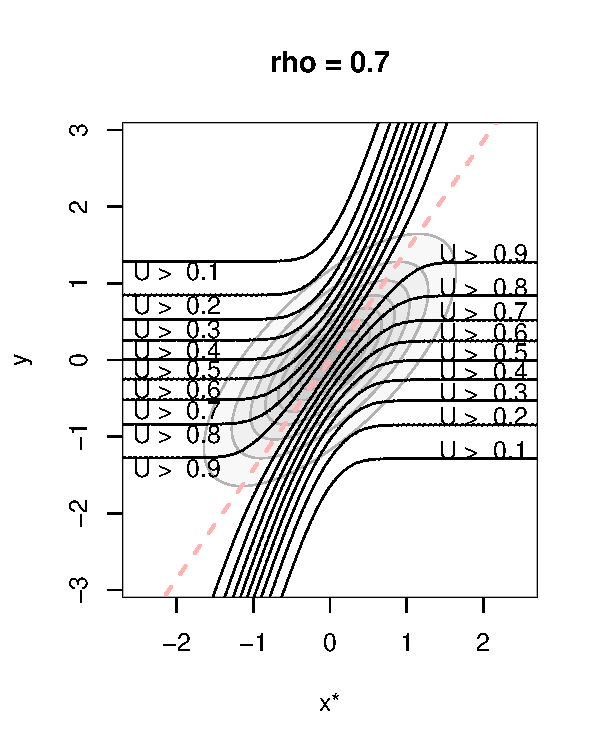
\includegraphics[scale = 0.6, clip = true, trim = 0.1in 0 0 0.8in]{illus_ufunc_0_7.pdf} &
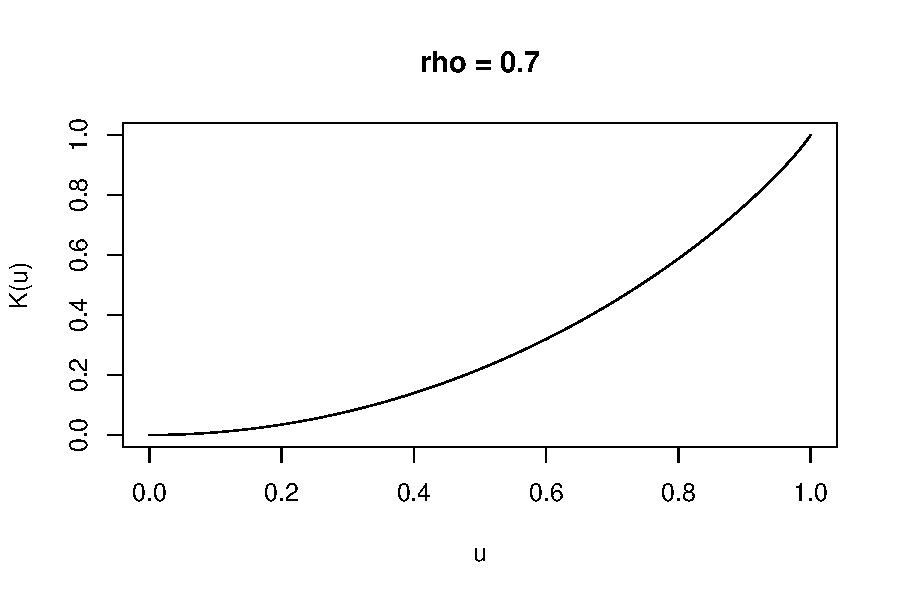
\includegraphics[scale = 0.65, clip = true, trim = 0 -0.3in 0 0.5in]{illus_kfunc_0_7.pdf}\\
(a) & (b)
\end{tabular}

\caption{
(a) The level curves of the function $U_x(y)$ in the bivariate normal model with $\rho = 0.7$.
(b) The function $\bar{D}(u)$, which gives the cumulative distribution function of the random variable $U_Y(X)$.}\label{fig:toy3}
\end{figure}

It is illuminating to consider how the average risk curves and the
$\bar{D}(u)$ functions vary as we change the parameter $\rho$.  Higher
correlations $\rho$ lead to lower classification risk, as seen in
figure \ref{fig:toy4}(a), where the risk curves are shifted downward as
$\rho$ increases from 0.3 to 0.9.  The conditional accuracy $U_y(x)$
tends to be higher on average as well, which leads to lower values of
the cumulative distribution function--as we see in
figure \ref{fig:toy4}(b), where the function $\bar{D}(u)$ becomes smaller
as $\rho$ increases.

In section \ref{sec:estimation}, when we consider approximating
$\bar{D}(u)$ by polynomials, or some other function basis, it becomes
relevant to consider how well $\bar{D}(u)$ can be approximated by such
bases in realistic problems.  We see in figure \ref{fig:toy4}(c) that,
at least in this toy problem, $\bar{D}(u)$ is well-aproximated by
low-order polynomials.  However, the approximation becomes less
adequate as $\rho$ increases.  We can see visually why this is the
case: as $\rho$ increases, the curvature of $\bar{D}(u)$ near $u = 1$
increases.  Hence, higher-degree polynomials become needed to capture
the behavior near $u = 1$.  More generally, we observe that in cases
where classes are relatively well-separated, it becomes necessary to
use increasingly precise approximations in order to extrapolate the
average risk.

\begin{figure}[h]
\centering
\begin{tabular}{ccc}
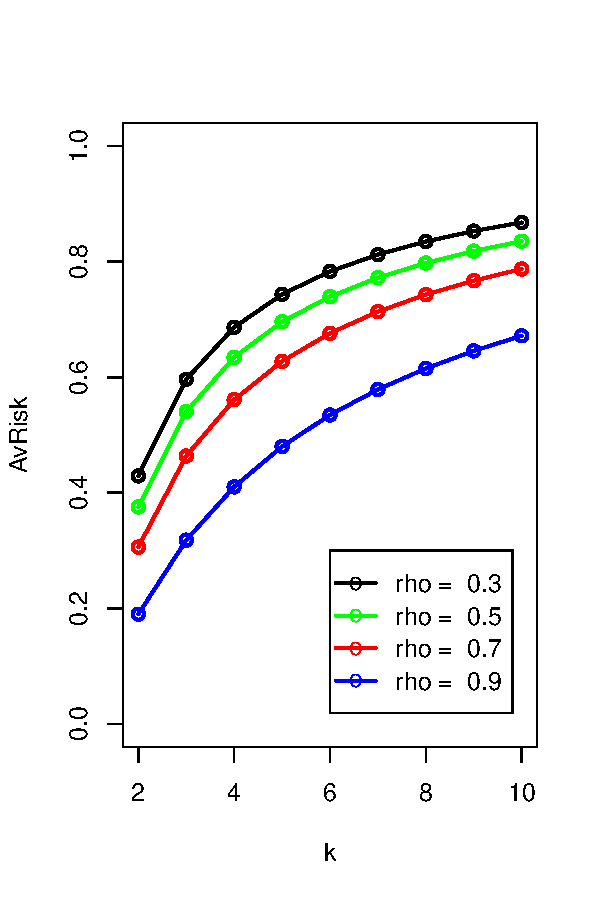
\includegraphics[scale = 0.45, clip = true, trim = 0.05in 0 0.2in 0.6in]{illus_rhos_avrisk.pdf} &
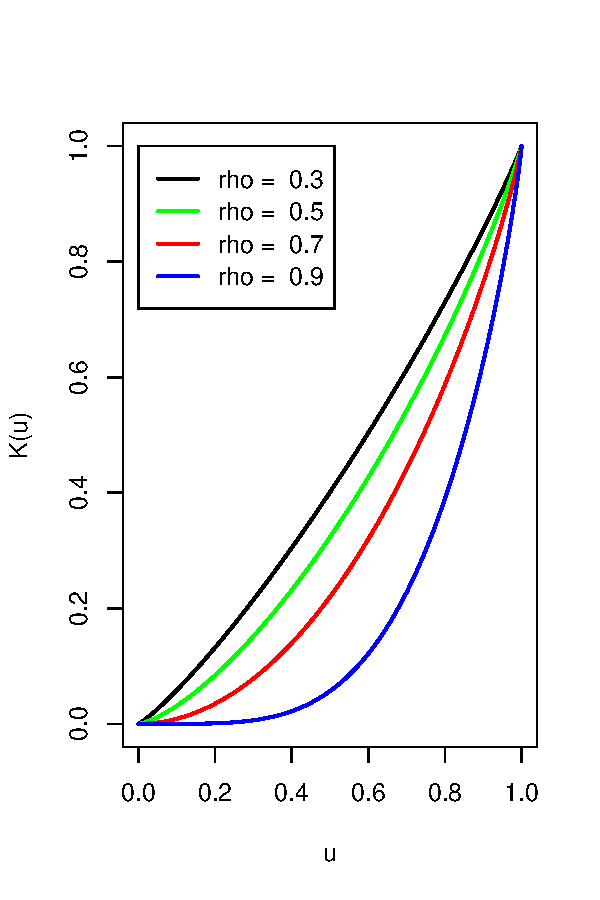
\includegraphics[scale = 0.45, clip = true, trim = 0.05in 0 0.2in 0.6in]{illus_rhos_Kfunc.pdf} &
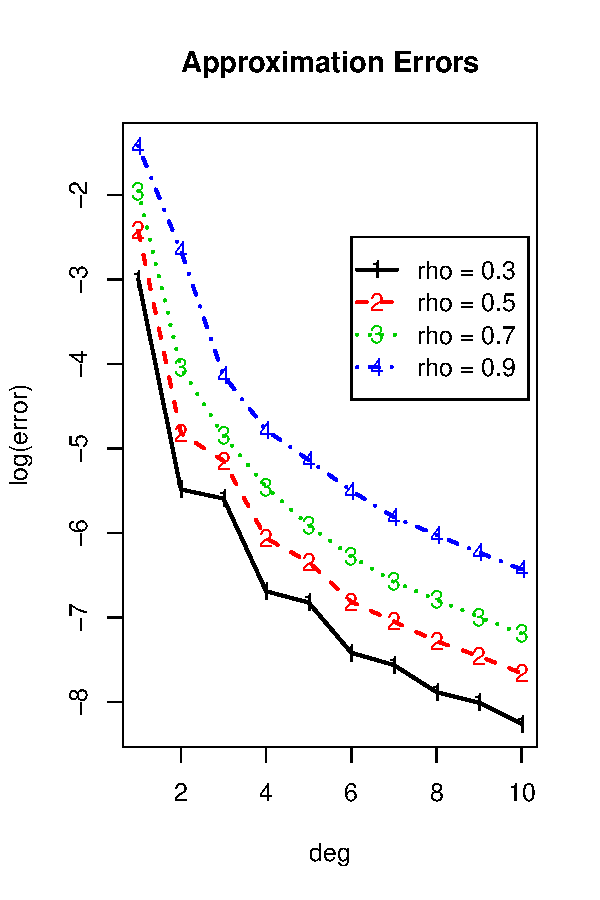
\includegraphics[scale = 0.45, clip = true, trim = 0.05in 0 0.2in 0.6in]{illus_approx_errors.pdf}\\
(a) & (b) & (c)
\end{tabular}

\caption{
The (a) average risk, (b) $\bar{D}(u)$ function for $k = 2,\hdots, 7$ for the bivariate normal model with $\rho \in \{0.3, 0.5, 0.7, 0.9\}$.
(c) The $d$-degree $\ell_\infty$ polynomial approximation error for $\bar{D}(u)$ for the bivariate normal model with $\rho \in \{0.3, 0.5, 0.7, 0.9\}$.
}\label{fig:toy4}
\end{figure}


\section{Examples}\label{sec:extrapolation_example}

\subsection{Facial recognition example}

From the ``Labeled Faces in the Wild'' dataset (\cite{LFWTech}), we
selected 1672 individuals with at least 2 face photos.  We form a
dataset consisting of photo-label pairs $(\vec{z}_j^{(i)}, y^{(i)})$
for $i = 1,\hdots, 1672$ and $j = 1,2$ by randomly selecting 2 face
photos for each of the 1672 individuals.

We implement a face recognition system based on one nearest-neighbor
and OpenFace (\cite{amos2016openface}) for feature extraction.  For
each photo $\vec{z}$, a 128-dimensional feature vector $\vec{x}$ is
obtained as follows.
\begin{enumerate}
\item The computer vision library DLLib is used to detect landmarks in
  $\vec{z}$, and to apply a nonlinear transformation to align
  $\vec{z}$ to a template.
\item The aligned photograph is downsampled to a $96 \times 96$ input,
  which is fed into a pre-trained deep convolutional neural network to
  obtain the 128-dimensional feature vector $\vec{x}$.
\end{enumerate}
Therefore, we obtain feature-label pairs $(\vec{x}_j^{(i)}, y^{(i)})$
for $i = 1,\hdots, 1672$ and $j = 1,2$.

The recognition system then works as follows.  Suppose we want to
perform facial recognition on a subset of the individuals, $I \subset
\{1,\hdots, 1672\}$.  Then, for all $i \in I$, we load one feature
vector-label pair, into the system, $(\vec{x}_1^{(i)}, y^{(i)})$.  In
order to identify a new photo $\vec{z}^*$, we obtain the feature
vector $\vec{x}^*$, and guess the label $\hat{y}$ based on example
with the minimal distance to $\vec{x}^*$,
\[
\hat{y} = y^{(i^*)}
\]
where
\[
i^* = \text{argmin}_i d(\vec{x}, \vec{x}_1^{(i)}).
\]
The test accuracy is assessed on the unused repeat for all individuals
in $I$.  Note that the assumptions of our estimation method are met in
this example because one-nearest neighbor is a marginal classifier.
One can define the score functions as
\[
(\mathcal{M}(\vec{x}))(\vec{x}^*) = -||\vec{x} - \vec{x}^*||^2.
\]
We note that $m$-nearest neighbor for $m > 1$ is not marginal.

While we can apply our extrapolation method to estimate the average
accuracy for any number of faces $k$, it will not be possible to
validate our estimates if we use the full dataset.  Therefore, we take
the average accuracies computed using the subsampling method
\eqref{eq:avtestrisk} on the full dataset as a \emph{ground truth} to
compare to the average accuracy estimated from a \emph{subsampled}
dataset.  Therefore, we simulate the problem of performance
extrapolation from a database of $K$ faces by subsampling a
dataset of size $K$ from the LFW dataset.

\begin{figure}
\centering
\begin{tabular}{cc}
a & b\\
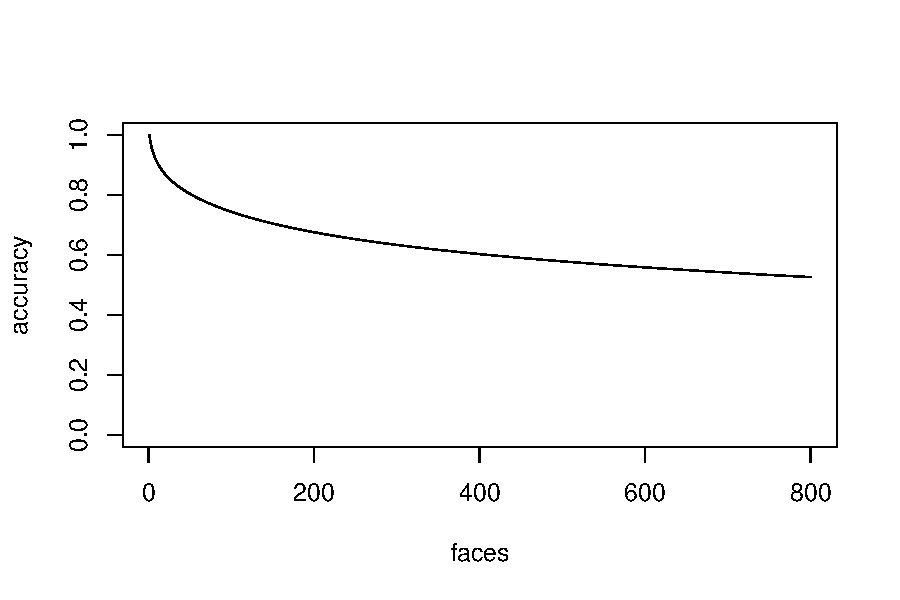
\includegraphics[scale = 0.5]{acc_plot1.pdf} &
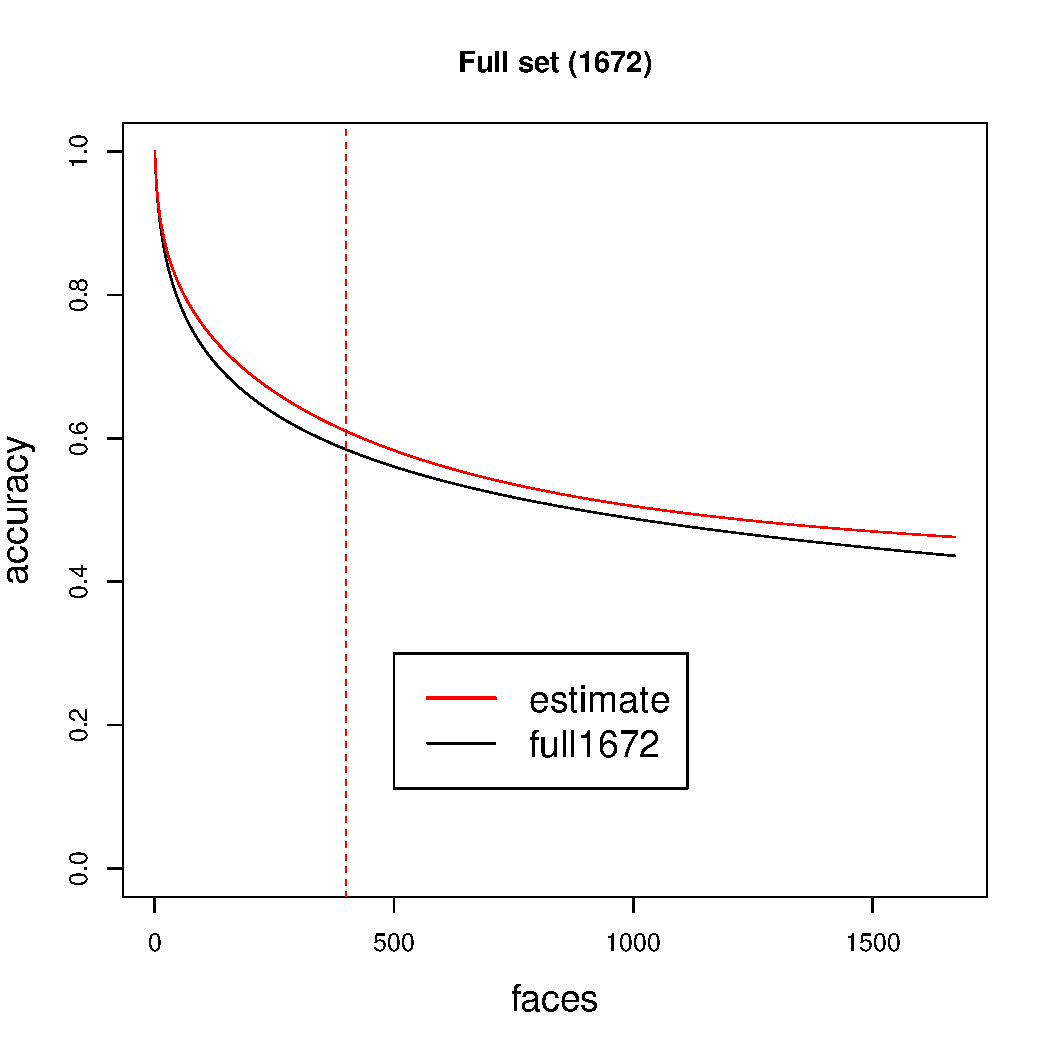
\includegraphics[scale = 0.5]{acc_plot2.pdf}
\end{tabular}
\caption{(a) The estimated average accuracy for $k = 2,\hdots,
  400$ given a dataset of 400 faces subsampled from Labeled Faces in
  the Wild.  (b) Estimated average accuracy for $k > 400$ on the
  same dataset, compared to the ground truth (average $k$-class test accuracy
  using all 1672 classes).}
\label{fig:lfw_extrapolation1}
\end{figure}

To do the performance extrapolation, we use a linear
spline basis,
\[
h_\ell(u) = \left[u - \frac{\ell - 1}{m}\right]_+
\]
for $\ell = 1,\hdots, m$.  Here we take $m = 10000$.  We model the
function $\bar{D}(u)$ as a non-negative linear combination of basis
functions,
\[
\bar{D}(u) = \sum_{\ell = 1}^m \beta_\ell h_\ell(u),
\]
with $\beta_\ell \geq 0$.  The non-negativity constraint on the
coefficients $\beta$, combined with the linear spline basis, ensures
that $\bar{D}(u)$ is a monotonic and convex function on $[0,1]$.  We
have found that in many simulated examples, $D(u)$ appears to be
monotone and convex, and we have also found that including the
monotonicity and convexity constraint in the estimation procedure
improves performance in practical examples.  The resulting estimated
generalization accuracies, computed using \eqref{eq:avrisk_identity},
are plotted in Figure \eqref{fig:lfw_extrapolation1} (b).  As we
already mentioned, to assess the quality of the estimated average
accuracy, we compare them to the `ground truth' accuracy curve
obtained by using all 1672 examples to compute the the average test
risk.




To get an idea of the accuracy and variance of the accuracy curve
estimates for varying sample sizes $K$, we repeat this procedure
multiple times for $K \in \{100,200,400, 800\}$.  The results, again
compared to the ground truth computed from the full data set, are
illustrated in figure \ref{fig:lfw_extrapolation2}.

\begin{figure}
\centering
\begin{tabular}{cc}
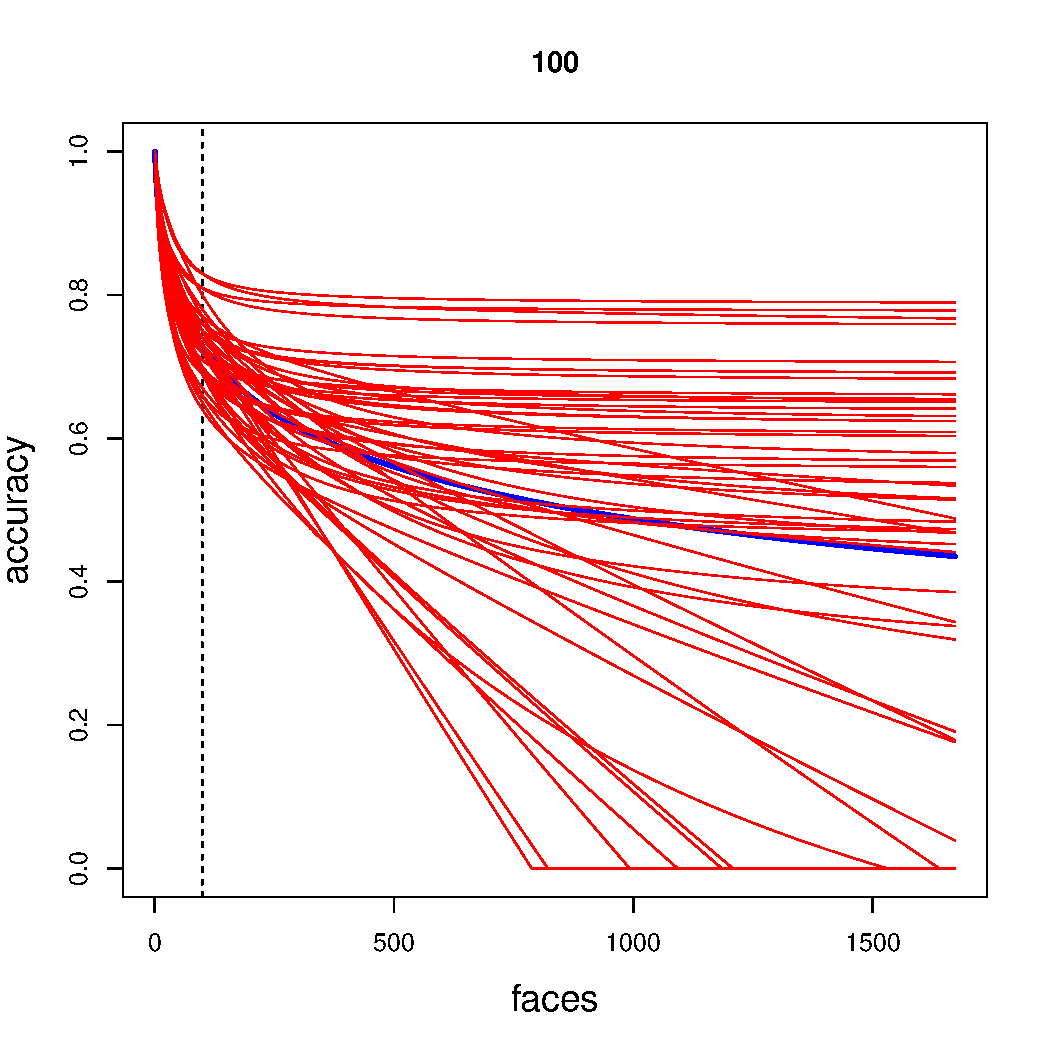
\includegraphics[scale = 0.4]{sub_100.pdf} &
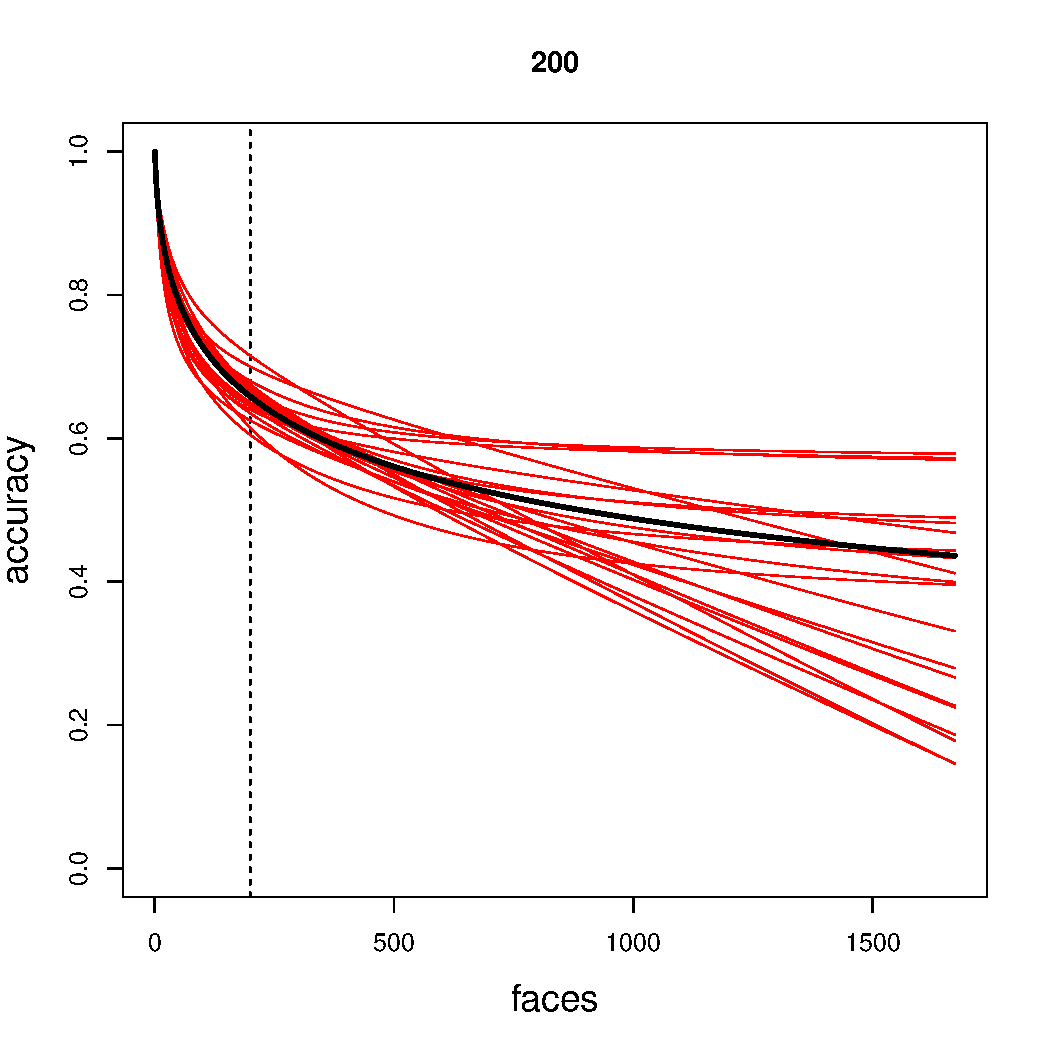
\includegraphics[scale = 0.4]{sub_200.pdf} \\
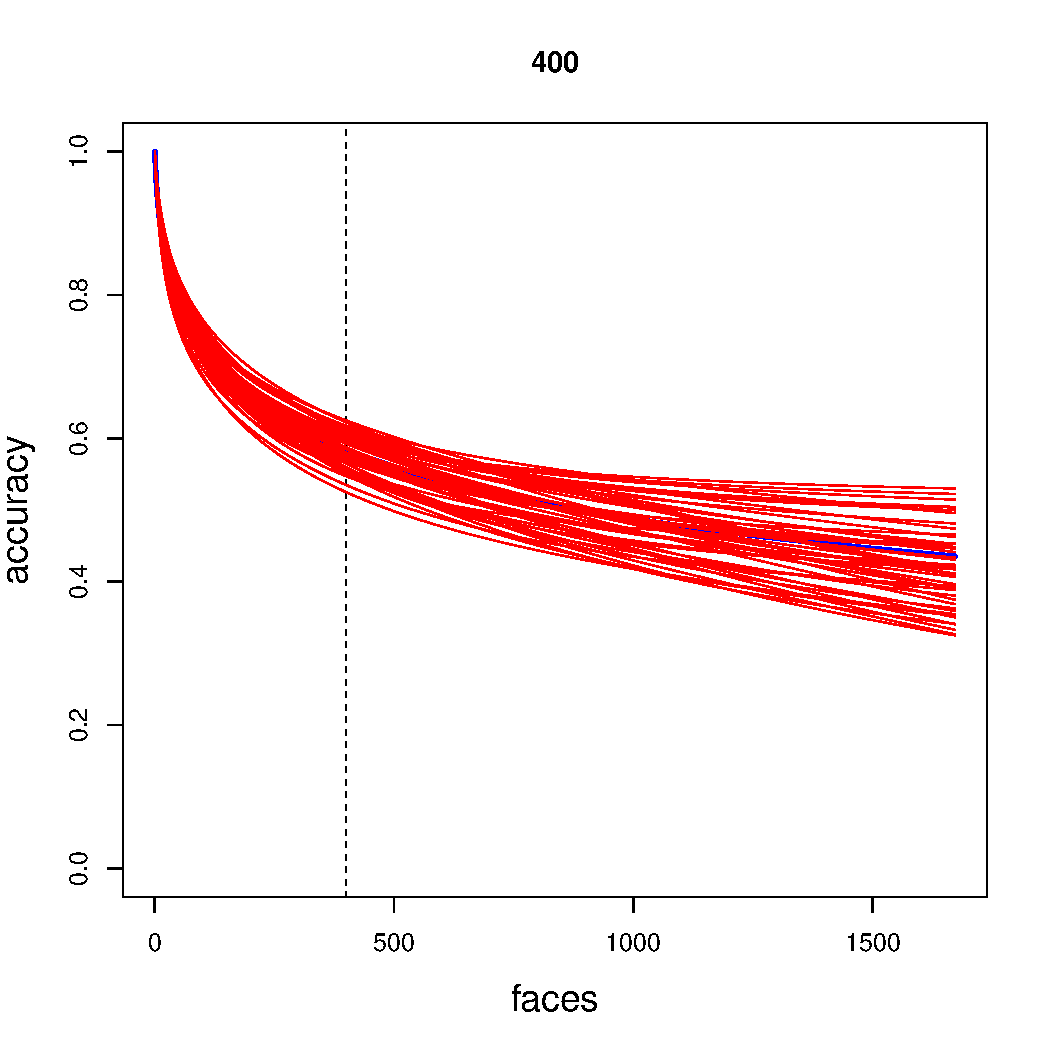
\includegraphics[scale = 0.4]{sub_400.pdf} &
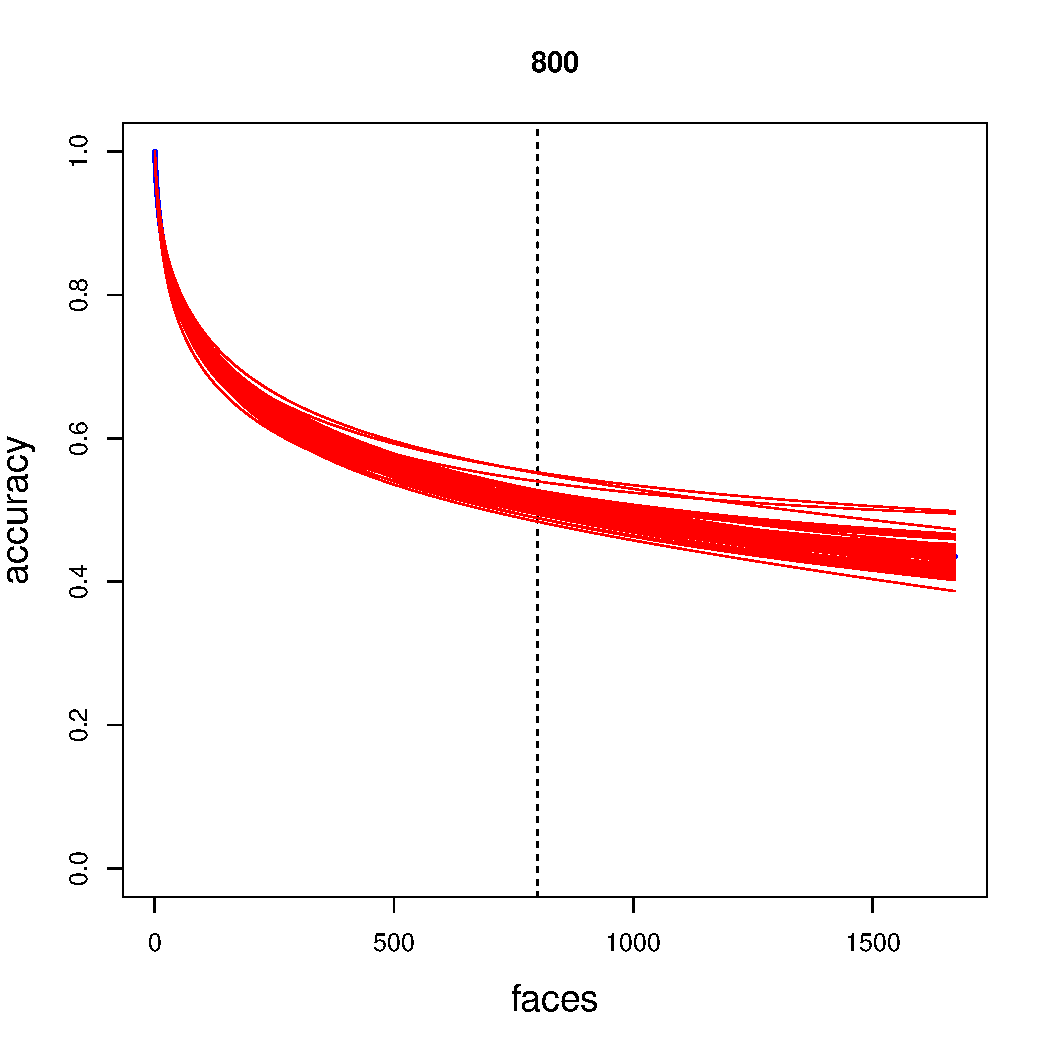
\includegraphics[scale = 0.4]{sub_800.pdf} 
\end{tabular}
\caption{Estimated average accuracy using subsampled datasets of size
  $k$, compared to the ground truth (average $k$-class test accuracy
  using all 1672 classes).}
\label{fig:lfw_extrapolation2}
\end{figure}


While further work is still needed to better understand the
performance of the proposed performance extrapolation method, both for
marginal classifiers (which satisfy the theoretical assumptions) and
non-marginal classifiers (which do not), the results obtained in these
two examples are encouraging in that sense that useful predictions
were obtained both for marginal and non-marginal classifiers.

\section{Discussion}

\printbibliography[heading=bibintoc]

\end{document}






















